\PassOptionsToPackage{table}{xcolor}
\documentclass[10pt,aspectratio=169]{beamer}

\usetheme[numbering=fraction]{metropolis}

\usepackage{booktabs}
\usepackage{tabularx}
\usepackage{makecell}
\usepackage{graphicx}
\usepackage{tikz}
\usepackage{xcolor}
\usepackage{colortbl}
\usepackage{pifont}
\usetikzlibrary{positioning}

\graphicspath{{assets/}}

\definecolor{SlideAccent}{HTML}{0B3D91}

% Report table style (mirrors report/preamble/preamble.tex)
\newcommand{\cmark}{\ding{51}}%
\newcommand{\xmark}{\ding{55}}%
\definecolor{gpuColor}{RGB}{217,234,211}     % D9EAD3
\definecolor{ggufColor}{RGB}{217,210,233}    % D9D2E9
\definecolor{axeleraColor}{RGB}{207,226,243} % CFE2F3
\definecolor{averageColor}{RGB}{230,230,230}
\definecolor{promptColor}{RGB}{255,242,204}  % FFF2CC
\definecolor{ragColor}{RGB}{244,204,204}     % F4CCCC
\definecolor{outputColor}{RGB}{201,218,248}  % C9DAF8

\setbeamercolor{alerted text}{fg=SlideAccent}
\setbeamercolor{progress bar}{fg=SlideAccent}
\setbeamercolor{title separator}{fg=SlideAccent}

% White background everywhere (including Metropolis title/frametitle bars)
\setbeamercolor{background canvas}{bg=white}
\setbeamercolor{normal text}{fg=black,bg=white}
\setbeamercolor{frametitle}{fg=black,bg=white}
\setbeamercolor{title}{fg=black,bg=white}

\title{RISCVxLLMxRobot}
\subtitle{Hybrid MPC+LLM decision-making on Axelera Metis: RAG, early stopping, quantization, and SFT}
\author{Facundo Garc\'ia C\'ardenas}
\date{\today}
\titlegraphic{\hfill\includegraphics[height=0.9cm]{eth_logo}}

\newcommand{\metric}[1]{\textbf{#1}}
\newcommand{\ok}{\textcolor{SlideAccent}{\textbf{✓}}}

\begin{document}

\maketitle

\begin{frame}{Agenda}
  \begin{itemize}
    \item Motivation \& goal
    \item DecisionxLLM task and evaluation setup
    \item Key results (RAG, early stopping, GGUF, Axelera INT8, SFT)
    \item Takeaways and next steps
  \end{itemize}
\end{frame}

\begin{frame}{Motivation}
  \begin{itemize}
    \item LLMs can add \alert{intent-aware reasoning} to autonomous driving, but must meet \alert{latency, memory, and energy} constraints.
    \item Hybrid stacks keep \alert{MPC} in charge of continuous control and safety constraints, and use the LLM as a \alert{decision/intent layer}.
    \item Embedded deployments should avoid cloud dependencies: \alert{on-board RAG} and efficient inference are key.
  \end{itemize}
\end{frame}

\begin{frame}{What is an ADS? (Autonomous Driving System)}
  \begin{itemize}
    \item An ADS is the full stack that turns \textbf{sensor inputs} (e.g., cameras/LiDAR/IMU) into \textbf{safe driving behavior}.
    \item Typical modules: perception $\rightarrow$ localization $\rightarrow$ prediction $\rightarrow$ planning $\rightarrow$ control.
    \item Key requirements: \textbf{safety}, \textbf{reliability}, \textbf{low latency}, and \textbf{robustness to edge cases}.
  \end{itemize}
\end{frame}

\begin{frame}{Why on-board? Why knowledge-driven?}
  \begin{itemize}
    \item \textbf{Autonomy implies on-board compute:} cloud calls add latency, reduce availability (coverage), and complicate safety guarantees.
    \item \textbf{Energy and memory are constrained} on embedded platforms; token generation directly impacts compute/energy.
    \item \textbf{Knowledge-driven reasoning complements data-driven policies:}
      \begin{itemize}
        \item adds human-interpretable rules/intent (e.g., “keep a safe distance”),
        \item improves generalization without requiring more training data for rare cases,
        \item can inject domain hints via on-board RAG without external connectivity.
      \end{itemize}
  \end{itemize}
\end{frame}

\begin{frame}{Related work I: on-board LLMs for ADS (Baumann et al., 2025)}
  \begin{itemize}
    \item \textbf{Core idea:} hybrid MPC+LLM architecture where the LLM operates at the \textbf{reasoning/intent layer} and MPC enforces feasibility.
    \item \textbf{DecisionxLLM:} classify whether recent driving behavior adheres to a language intent from short state histories.
    \item \textbf{RAG:} retrieve compact domain hints to improve decision quality without increasing model size.
    \item \textbf{Embedded focus:} emphasize on-board deployment constraints (latency/memory/energy) and quantized inference.
  \end{itemize}
  \vspace{0.5em}
  \footnotesize
  Nicolas Baumann et al., “Enhancing Autonomous Driving Systems with On-Board Deployed Large Language Models”, arXiv:2504.11514.\\
  \href{https://arxiv.org/abs/2504.11514}{https://arxiv.org/abs/2504.11514}
\end{frame}

\begin{frame}{Related work II: RobotxR1 (Boyle et al., 2025)}
  \begin{itemize}
    \item \textbf{Goal:} enable embodied robotic intelligence on compact LLMs through \textbf{closed-loop reinforcement learning}.
    \item \textbf{RLVR framing:} train models with \textbf{verifiable rewards} (e.g., formatting + correctness of structured outputs).
    \item \textbf{Relevance here:} motivates \textbf{binary decision heads} (verifiable, parseable) and robust formatting as a training target.
  \end{itemize}
  \vspace{0.5em}
  \footnotesize
  Liam Boyle et al., “RobotxR1: Enabling Embodied Robotic Intelligence on Large Language Models through Closed-Loop Reinforcement Learning”, arXiv:2505.03238.\\
  \href{https://arxiv.org/abs/2505.03238}{https://arxiv.org/abs/2505.03238}
\end{frame}

\begin{frame}{Goal \& scope}
  \begin{itemize}
    \item Port DecisionxLLM-style decision classification to Axelera Metis (INT8, vendor compiler/runtime).
    \item Benchmark on GPU FP16, GGUF (\texttt{llama.cpp}), and Axelera INT8 under identical prompts/datasets.
    \item Study:
      \begin{itemize}
        \item RAG: OpenAI embeddings vs on-board BGE embeddings
        \item Verifiable binary decision head + early stopping
        \item Quantization (GGUF) and compilation effects (Axelera INT8)
        \item SFT to improve robustness and formatting
      \end{itemize}
  \end{itemize}
\end{frame}

\begin{frame}{Contributions}
  \begin{itemize}
    \item End-to-end port of DecisionxLLM evaluation to an accelerator-centric stack (Axelera Metis).
    \item On-board RAG (BGE embeddings) benchmarked against a cloud OpenAI-embeddings baseline.
    \item Verifiable binary decision head + early stopping to reduce generation and energy cost.
    \item GGUF quantization study (e.g., Q4.M) via \texttt{llama.cpp} vs GPU FP16 baselines.
    \item Characterization of Axelera INT8 behavior (structure vs decision quality).
    \item Energy-aware profiling methodology for embedded comparisons (Axelera+SBC vs Jetson Orin AGX).
    \item SFT experiments to improve structural adherence and reduce verbosity.
  \end{itemize}
\end{frame}

\begin{frame}{Experiment matrix}
  \small
  \setlength{\tabcolsep}{5pt}
  \begin{tabularx}{\textwidth}{l X}
    \toprule
    \textbf{Axis} & \textbf{Variants} \\
    \midrule
    Task & DecisionxLLM adherence classification (8 driving behaviors) \\
    Backends & GPU FP16 (Transformers), GGUF Q4.M (\texttt{llama.cpp}), Axelera Metis INT8 \\
    RAG & none, OpenAI embeddings (cloud), BGE embeddings (on-board) \\
    Output mode & explanatory vs binary decision head (+ early stopping) \\
    Models & Phi-3 (3.8B), Llama (3.2B/8B), Qwen2.5 (3B/7B), SFT variants \\
    Metrics & structure-followed, avg/parsed accuracy, output tokens (power profiling WIP) \\
    \bottomrule
  \end{tabularx}
\end{frame}

\begin{frame}{Decision task (DecisionxLLM)}
  \begin{columns}[T,onlytextwidth]
    \column{0.62\textwidth}
      \begin{itemize}
        \item Input: \metric{human intent} + \metric{robot state window} in Frenet frame.
        \item State window contains sequences of:
          \begin{itemize}
            \item $s_\text{pos}, d_\text{pos}$ (track progress / lateral offset)
            \item $s_\text{speed}, d_\text{speed}$ (longitudinal / lateral speed)
            \item $d_\text{left}, d_\text{right}$ (distance to track boundaries)
          \end{itemize}
        \item Output: \metric{adherence} to intent (\texttt{True/False}) with optional explanation.
      \end{itemize}
    \column{0.38\textwidth}
      \vspace{-0.5em}
      \includegraphics[width=\linewidth]{rss_abstract_figure}
  \end{columns}
\end{frame}

\begin{frame}{Pipeline overview (backend-agnostic)}
  \centering
  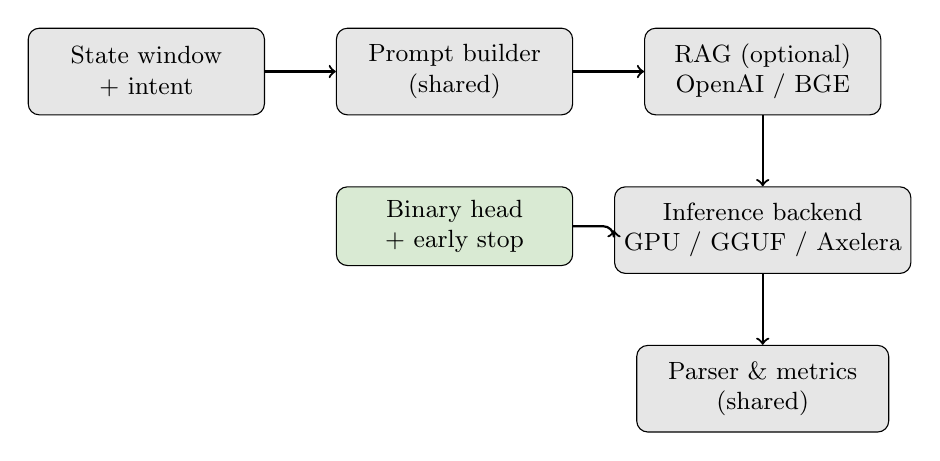
\begin{tikzpicture}[node distance=9mm, every node/.style={font=\small}, rounded corners]
    \node[draw, fill=averageColor, align=center, minimum width=3.0cm, minimum height=1.1cm] (data) {State window\\+ intent};
    \node[draw, fill=averageColor, right=of data, align=center, minimum width=3.0cm, minimum height=1.1cm] (prompt) {Prompt builder\\(shared)};
    \node[draw, fill=averageColor, right=of prompt, align=center, minimum width=3.0cm, minimum height=1.1cm] (rag) {RAG (optional)\\OpenAI / BGE};

    \node[draw, fill=averageColor, below=of rag, align=center, minimum width=3.2cm, minimum height=1.1cm] (backend) {Inference backend\\GPU / GGUF / Axelera};
    \node[draw, fill=averageColor, below=of backend, align=center, minimum width=3.2cm, minimum height=1.1cm] (parse) {Parser \& metrics\\(shared)};

    \node[draw, fill=gpuColor, below=of prompt, align=center, minimum width=3.0cm, minimum height=1.0cm] (binary) {Binary head\\+ early stop};

    \draw[->, thick] (data) -- (prompt);
    \draw[->, thick] (prompt) -- (rag);
    \draw[->, thick] (rag) -- (backend);
    \draw[->, thick] (backend) -- (parse);
    \draw[->, thick] (binary) -| (backend.west);
  \end{tikzpicture}
\end{frame}

\begin{frame}{Metrics}
  \begin{itemize}
    \item \metric{Structure-followed rate}: output matches schema (parseable).
    \item \metric{Average accuracy}: accuracy over all samples (malformed = incorrect).
    \item \metric{Parsed accuracy}: accuracy over parseable samples only.
    \item \metric{Token statistics}: prompt / RAG hint / output length (proxy for latency/energy).
  \end{itemize}
  \vspace{0.5em}
  \small
  In tables: accuracy shown as \texttt{avg | parsed}. Lower tokens are better.
\end{frame}

\begin{frame}{RAG on GPU: on-board BGE vs cloud OpenAI embeddings}
  \scriptsize
  \setlength{\tabcolsep}{6pt}
  \renewcommand{\arraystretch}{1.15}
  \begin{tabular}{lcccc}
    \toprule
    \multicolumn{5}{c}{\cellcolor{gpuColor} \textbf{GPU FP16 baselines (RAG comparison)}} \\
    \midrule
    \makecell{\textbf{Model}\\\textbf{name}} & \makecell{\textbf{RAG}\\\textbf{type}} & \makecell{\textbf{Struct}\\\textbf{(\%)}} & \makecell{\textbf{Accuracy}\\\textbf{(avg. | par.)}} & \makecell{\textbf{Out tok}\\\textbf{(avg.)}} \\
    \midrule
    Phi3 & \xmark & 99.18\% & 71.83 | 72.39\% & 114 \\
    Phi3 & OpenAI & 100.00\% & \textbf{79.31 | 79.31\%} & 150 \\
    Phi3 & BGE & 100.00\% & 77.86 | 77.86\% & 160 \\
    \midrule
    Llama3.2 & \xmark & 98.22\% & 70.75 | 72.10\% & 120 \\
    Llama3.2 & OpenAI & 97.21\% & 66.24 | 68.52\% & 124 \\
    Llama3.2 & BGE & \cellcolor{ragColor}86.42\% & 69.54 | \textbf{80.58\%} & \cellcolor{outputColor}227 \\
    \midrule
    Qwen2.5 (7B) & \xmark & 100.00\% & 81.35 | 81.35\% & 109 \\
    Qwen2.5 (7B) & OpenAI & 100.00\% & 84.33 | 84.33\% & 129 \\
    Qwen2.5 (7B) & BGE & 100.00\% & \textbf{86.55 | 86.55\%} & 124 \\
    \bottomrule
  \end{tabular}

  \vspace{0.7em}
  \footnotesize
  Takeaway: BGE (on-board) often matches the cloud retriever, but the effect depends on backbone and can interact with structure-followed rate.
\end{frame}

\begin{frame}{Why tokens matter (Phi-3 example)}
  \scriptsize
  \setlength{\tabcolsep}{6pt}
  \renewcommand{\arraystretch}{1.15}
  \begin{tabular}{lccc}
    \toprule
    \multicolumn{4}{c}{\cellcolor{gpuColor} \textbf{Token-length summary (Phi-3, GPU)}} \\
    \midrule
    \textbf{Metric (mean)} & \textbf{No RAG} & \textbf{OpenAI RAG} & \textbf{BGE RAG} \\
    \midrule
    \rowcolor{promptColor} Prompt tokens & 607.3 & 762.8 & 751.3 \\
    \rowcolor{ragColor} RAG hint tokens & 0.0 & 156.5 & 145.0 \\
    \rowcolor{outputColor} Output tokens & 115.1 & 150.9 & 158.7 \\
    \rowcolor{averageColor} \textbf{Context tokens} & \textbf{722.4} & \textbf{913.7} & \textbf{910.0} \\
    \bottomrule
  \end{tabular}

  \vspace{0.7em}
  \footnotesize
  Takeaway: decoding cost scales with generated output tokens; early stopping targets the most controllable term.
\end{frame}

\begin{frame}{Phi-3 per-behavior accuracy (GPU)}
  \scriptsize
  \setlength{\tabcolsep}{7pt}
  \renewcommand{\arraystretch}{1.15}
  \begin{tabular}{lccc}
    \toprule
    \multicolumn{4}{c}{\cellcolor{gpuColor} \textbf{Per-behavior accuracy (Phi-3, GPU)}} \\
    \midrule
    \textbf{Behavior} & \textbf{No RAG} & \textbf{OpenAI RAG} & \textbf{BGE RAG} \\
    \midrule
    Centerline    & 83.15\% & 91.85\% & 84.24\% \\
    Close to wall & 56.50\% & 68.00\% & 59.00\% \\
    Forward       & 76.00\% & 82.50\% & 77.50\% \\
    Oscillating   & 77.00\% & 83.00\% & 79.50\% \\
    Racingline    & 72.00\% & 79.50\% & 79.00\% \\
    Reversed      & 49.48\% & 66.67\% & \textbf{79.17\%} \\
    Speed         & 75.00\% & 77.00\% & 77.00\% \\
    Stop          & 86.00\% & 85.50\% & 85.00\% \\
    \midrule
    \rowcolor{averageColor}
    \textbf{Average} & \textbf{71.89\%} & \textbf{79.25\%} & \textbf{77.55\%} \\
    \bottomrule
  \end{tabular}

  \vspace{0.7em}
  \footnotesize
  Takeaway: RAG helps most on hard cases (e.g., \textit{Reversed}) while leaving easy behaviors largely unchanged.
\end{frame}

\begin{frame}{Binary decision head + early stopping (GPU)}
  \scriptsize
  \setlength{\tabcolsep}{6pt}
  \renewcommand{\arraystretch}{1.15}
  \begin{tabular}{lcccccc}
    \toprule
    \multicolumn{7}{c}{\cellcolor{gpuColor} \textbf{Binary decision head with early stopping (GPU)}} \\
    \midrule
    \makecell{\textbf{Model}\\\textbf{name}} & \makecell{\textbf{Model}\\\textbf{Params}} & \makecell{\textbf{RAG}\\\textbf{type}} & \makecell{\textbf{Binary}\\\textbf{output}} & \makecell{\textbf{Struct}\\\textbf{(\%)}} & \makecell{\textbf{Accuracy}\\\textbf{(avg. | par.)}} & \makecell{\textbf{Tokens}\\\textbf{(avg. | par.)}} \\
    \midrule
    Phi3 & 3.80 B & \xmark & \xmark & 99.18\% & \hphantom{}71.83 | 72.39\hphantom{}\% & \hphantom{}114 | 111\hphantom{} \\
    Phi3 & 3.80 B & \xmark & \cmark & 100.00\% & \hphantom{}70.88 | 70.88\hphantom{}\% & \hphantom{00}7 | 7\hphantom{00} \\
    \addlinespace
    Qwen2.5 & 7.61 B & \xmark & \xmark & 100.00\% & \hphantom{}81.35 | 81.35\hphantom{}\% & \hphantom{}109 | 109\hphantom{} \\
    Qwen2.5 & 7.61 B & \xmark & \cmark & 100.00\% & \hphantom{}81.47 | 81.47\hphantom{}\% & \hphantom{00}7 | 7\hphantom{00} \\
    \bottomrule
  \end{tabular}
\vspace{0.7em}
\footnotesize{Takeaway: binary outputs reduce generation from $\sim$100+ tokens to 7 with minimal accuracy change (when structure is followed).}
\end{frame}

\begin{frame}{Binary head: what it enables}
  \begin{itemize}
    \item \textbf{Verifiable output:} single-line decision is easy to parse and score.
    \item \textbf{Early stopping:} stop as soon as the decision is produced (avoid long explanations).
    \item \textbf{Efficiency:} token reduction typically yields lower latency and energy per decision.
    \item \textbf{Robustness lever:} if structure-followed drops, average accuracy collapses even if parsed accuracy is high.
  \end{itemize}
\end{frame}

\begin{frame}{GGUF quantization (Q4.M vs Q5.M, \texttt{llama.cpp})}
  \scriptsize
  \setlength{\tabcolsep}{6pt}
  \renewcommand{\arraystretch}{1.15}
  \begin{tabular}{lcccccc}
    \toprule
    \multicolumn{7}{c}{\cellcolor{ggufColor} \textbf{GGUF quantization (Q4.M/Q5.M) vs GPU FP16}} \\
    \midrule
    \makecell{\textbf{Model}\\\textbf{name}} & \makecell{\textbf{Model}\\\textbf{Params}} & \makecell{\textbf{RAG}\\\textbf{type}} & \makecell{\textbf{Device}\\\textbf{used}} & \makecell{\textbf{Struct}\\\textbf{(\%)}} & \makecell{\textbf{Accuracy}\\\textbf{(avg. | par.)}} & \makecell{\textbf{Tokens}\\\textbf{(avg. | par.)}} \\
    \midrule
    Phi3 & 3.80 B & BGE & GPU (FP16) & 100.00\% & \hphantom{}77.86 | 77.86\hphantom{}\% & \hphantom{}160 | 160\hphantom{} \\
    Phi3 & 3.80 B & BGE & GGUF (Q4.M) & 99.81\% & \hphantom{}71.95 | 72.06\hphantom{}\% & \hphantom{0}63 | 63\hphantom{0} \\
    Phi3 & 3.80 B & BGE & GGUF (Q5.M) & 100.00\% & \hphantom{}81.73 | 81.73\hphantom{}\% & \hphantom{}174 | 174\hphantom{} \\
    \addlinespace
    Llama3.2 & 3.21 B & \xmark & GPU (FP16) & 98.22\% & \hphantom{}70.75 | 72.10\hphantom{}\% & \hphantom{}120 | 113\hphantom{} \\
    Llama3.2 & 3.21 B & \xmark & GGUF (Q4.M) & 99.49\% & \hphantom{}66.43 | 66.78\hphantom{}\% & \hphantom{}185 | 184\hphantom{} \\
    Llama3.2 & 3.21 B & \xmark & GGUF (Q5.M) & 99.11\% & \hphantom{}66.94 | 67.61\hphantom{}\% & \hphantom{}104 | 101\hphantom{} \\
    \bottomrule
  \end{tabular}
\vspace{0.7em}
\footnotesize{Takeaway: Q4.M preserves structure but can shift accuracy and output length depending on backbone and prompts.}
\end{frame}

\begin{frame}{GGUF vs GPU: how to interpret}
  \begin{itemize}
    \item \textbf{Strength:} strong compression and fast local runtimes with high structure-followed rates.
    \item \textbf{Tradeoff:} accuracy and verbosity can shift depending on backbone and prompt template.
    \item \textbf{Recommendation:} benchmark the exact prompt + output mode (binary vs explanatory) you plan to deploy.
  \end{itemize}
\end{frame}

\begin{frame}{Axelera Metis (INT8): structure vs decision quality}
  \scriptsize
  \setlength{\tabcolsep}{6pt}
  \renewcommand{\arraystretch}{1.15}
  \begin{tabular}{lcccccc}
    \toprule
    \multicolumn{7}{c}{\cellcolor{axeleraColor} \textbf{Axelera Metis INT8 vs GPU baseline}} \\
    \midrule
    \makecell{\textbf{Model}} & \makecell{\textbf{Device}} & \makecell{\textbf{RAG}\\\textbf{type}} & \makecell{\textbf{Binary}\\\textbf{output}} & \makecell{\textbf{Struct}\\\textbf{(\%)}} & \makecell{\textbf{Accuracy}\\\textbf{(avg. | par.)}} & \makecell{\textbf{Tokens}\\\textbf{(avg. | par.)}} \\
    \midrule
    Phi3 (3.8B) & GPU (FP16) & \xmark & \xmark & 99.18\% & \hphantom{}71.83 | 72.39\hphantom{}\% & \hphantom{}114 | 111\hphantom{} \\
    Phi3 (3.8B) & Axelera (INT8) & \xmark & \xmark & 97.02\% & \hphantom{}55.84 | 57.54\hphantom{}\% & \hphantom{}223 | 221\hphantom{} \\
    Phi3 (3.8B) & Axelera (INT8) & \xmark & \cmark & 98.41\% & \hphantom{}66.12 | 67.09\hphantom{}\% & \hphantom{00}9 | 7\hphantom{00} \\
    \addlinespace
    Llama3.2 (3.2B) & GPU (FP16) & BGE & \xmark & 86.42\% & \hphantom{}69.54 | 80.58\hphantom{}\% & \hphantom{}227 | 184\hphantom{} \\
    Llama3.2 (3.2B) & Axelera (INT8) & BGE & \xmark & 49.62\% & \hphantom{}34.33 | 67.62\hphantom{}\% & \hphantom{}188 | 179\hphantom{} \\
    Llama3.2 (3.2B) & Axelera (INT8) & BGE & \cmark & 100.00\% & \hphantom{}52.98 | 52.98\hphantom{}\% & \hphantom{00}7 | 7\hphantom{00} \\
    \bottomrule
  \end{tabular}
\vspace{0.7em}
\footnotesize{Takeaway: Metis INT8 keeps structure relatively high, but decision accuracy can drop significantly (especially with RAG).}
\end{frame}

\begin{frame}{Axelera INT8: likely failure mode (hypothesis)}
  \begin{itemize}
    \item The same prompts/parsers produce strong structure-followed rates, but accuracy drops under Metis INT8.
    \item This suggests the bottleneck is \textbf{vendor quantization / compilation} rather than prompt wording.
    \item RAG can amplify the issue: hint conditioning may be more sensitive to quantization noise.
    \item Practical next step: tune calibration / compiler settings and re-check per-behavior errors.
  \end{itemize}
\end{frame}

\begin{frame}{SFT improves structure and reduces verbosity (Qwen2.5)}
  \scriptsize
  \setlength{\tabcolsep}{6pt}
  \renewcommand{\arraystretch}{1.15}
  \begin{tabular}{lccccc}
    \toprule
    \multicolumn{6}{c}{\cellcolor{gpuColor} \textbf{Effect of SFT on Qwen2.5 (GPU FP16, no-RAG)}} \\
    \midrule
    \makecell{\textbf{Model}\\\textbf{name}} & \makecell{\textbf{SFT}\\\textbf{}} & \makecell{\textbf{Binary}\\\textbf{output}} & \makecell{\textbf{Struct}\\\textbf{(\%)}} & \makecell{\textbf{Accuracy}\\\textbf{(avg. | par.)}} & \makecell{\textbf{Tokens}\\\textbf{(avg. | par.)}} \\
    \midrule
    Qwen2.5 (7.61B) & \xmark & \xmark & 100.00\% & \hphantom{}81.35 | 81.35\hphantom{}\% & \hphantom{}109 | 109\hphantom{} \\
    Qwen2.5 (7.61B) & \cmark & \xmark & 100.00\% & \hphantom{}85.28 | 85.28\hphantom{}\% & \hphantom{0}71 | 71\hphantom{0} \\
    Qwen2.5 (7.61B) & \cmark & \cmark & 100.00\% & \hphantom{}85.72 | 85.72\hphantom{}\% & \hphantom{00}7 | 7\hphantom{00} \\
    \bottomrule
  \end{tabular}
\vspace{0.7em}
\footnotesize{Takeaway: SFT maintains strong accuracy while improving verbosity/formatting; in binary mode it reliably emits a short decision.}
\end{frame}

\begin{frame}{Conclusion: problem context}
  \begin{itemize}
    \item \textbf{Goal:} enable knowledge-driven, language-conditioned decision-making in an ADS-like stack \textbf{fully on-board}.
    \item \textbf{Constraint:} no reliance on remote computation; embedded platforms have tight \textbf{latency, memory, and energy} budgets.
    \item \textbf{Question:} can we keep decision quality while porting the workload to heterogeneous backends (GPU, GGUF, Axelera INT8)?
  \end{itemize}
\end{frame}

\begin{frame}{Conclusion: findings \& next steps}
  \begin{itemize}
    \item On-board RAG (BGE) can recover much of cloud RAG’s benefit while remaining self-contained.
    \item Binary decision heads + early stopping are a high-leverage knob for embedded latency/energy.
    \item GGUF quantization is a practical path to smaller footprints with moderate accuracy shifts.
    \item Axelera INT8 shows strong structure but inconsistent decision quality: vendor quantization/compiler pipeline matters.
    \item Next: finish power profiling (energy/decision), and tune INT8 compilation for decision robustness.
  \end{itemize}
  \vfill
  \footnotesize
  Repository: \texttt{github.com/fgarciacardenas/RISCVxLLMxRobot}
\end{frame}

\end{document}
